\section{IoTeX: Panoramica sull'Architettura e il Progetto}

\subsection{Principio di progettazione}
IoTeX mira a diventare la spina dorsale ed il sistema nervoso dedicato all'IoT, scalabile e incentrato sulla privacy. Per raggiungere questo obiettivo e affrontare le sfide citate, il design della nostra architettura è basato sui seguenti princìpi.

\subsubsection{Separazione delle responsabilità}
Connettere direttamente tutti i nodi IoT in una singola blockchain è un sogno che non può essere realizzato. Oltre al fatto che le diverse applicazioni IoT richiedono fondamentalmente diversi insiemi di funzionalità della blockchain, ospitare ogni nodo IoT sulla stessa blockchain la farebbe comunque crescere rapidamente in dimensioni e in richieste computazionali, e alla fine diventerebbe troppo pesante per la maggior parte dei dispositivi IoT. Invece, una separazione delle funzioni assicura che ogni blockchain interagisca con un gruppo specifico di nodi IoT e, allo stesso tempo, interagisca con altre blockchain quando necessario. Analogamente a quanto accade per Internet, dispositivi eterogenei prima formano un gruppo interconnesso, la intranet; intranet più piccole possono ulteriormente formare una intranet più grande, che alla fine si connette alla spina dorsale di internet e tutti i dispositivi comunicano l'un l'altro.
La "Separazione delle responsabilità" di solito crea un sistema ben bilanciato, per massimizzare sia l'efficienza che la privacy.

\subsubsection{Il Rasoio di Occam}
Diverse blockchain hanno utilizzi e applicazioni diverse, e dovrebbero essere progettate e ottimizzate verso direzioni diverse. Ad esempio: una blockchain dedicata all'inoltro delle transazioni tra le sue subchain non necessita che su di essa vengano eseguiti smart-contract Turing-Completi; un'altra blockchain che colleghi dispositivi appartenenti alla stessa zona di fiducia non dovrebbe preoccuparsi troppo della privacy delle transazioni.

\subsubsection{Adatta per l'IoT}
Come già detto, il mondo IoT è pieno di sistemi e nodi eterogenei, più o meno potenti in termini di risorse di calcolo, archiviazione e alimentazione. Dal momento che le operazioni eseguibili dai nodi deboli possono comunque essere facilmente eseguite da quelli forti, le operazioni sulla blockchain dovrebbero essere progettate e ottimizzate per i nodi deboli, ovvero le operazioni dovrebbero essere abbastanza leggere da risparmiare risorse come potenza di calcolo, spazio di archiviazione ed energia.

\subsection{Architettura: Blockchain in Blockchain}
IoTeX è una rete di molte blockchain disposte gerarchicamente, dove molte blockchain possono funzionare parallelamente tra loro pur mantenendo l'interoperabilità. Nel mondo IoTeX, come mostrato nella Figura \ref{fig:fig1}, la blockchain radice (\emph{rootchain}) gestisce molte blockchain indipendenti, o \emph{subchain}. Una subchain si connette e interagisce con quei dispositivi IoT con i quali ha qualcosa in comune, ad esempio che hanno uno scopo funzionale simile, che operano in ambienti simili, o che condividono un livello di fiducia simile. Se una subchain non funziona bene, ad esempio se viene attaccata o si verificano bug del software, la rootchain rimane completamente inalterata. Inoltre, sono supportate transazioni tra blockchain per trasferire valore e dati dalle subchain alla rootchain, oppure tra una subchain e l'altra attraverso la rootchain.

\begin{figure}[ht]
	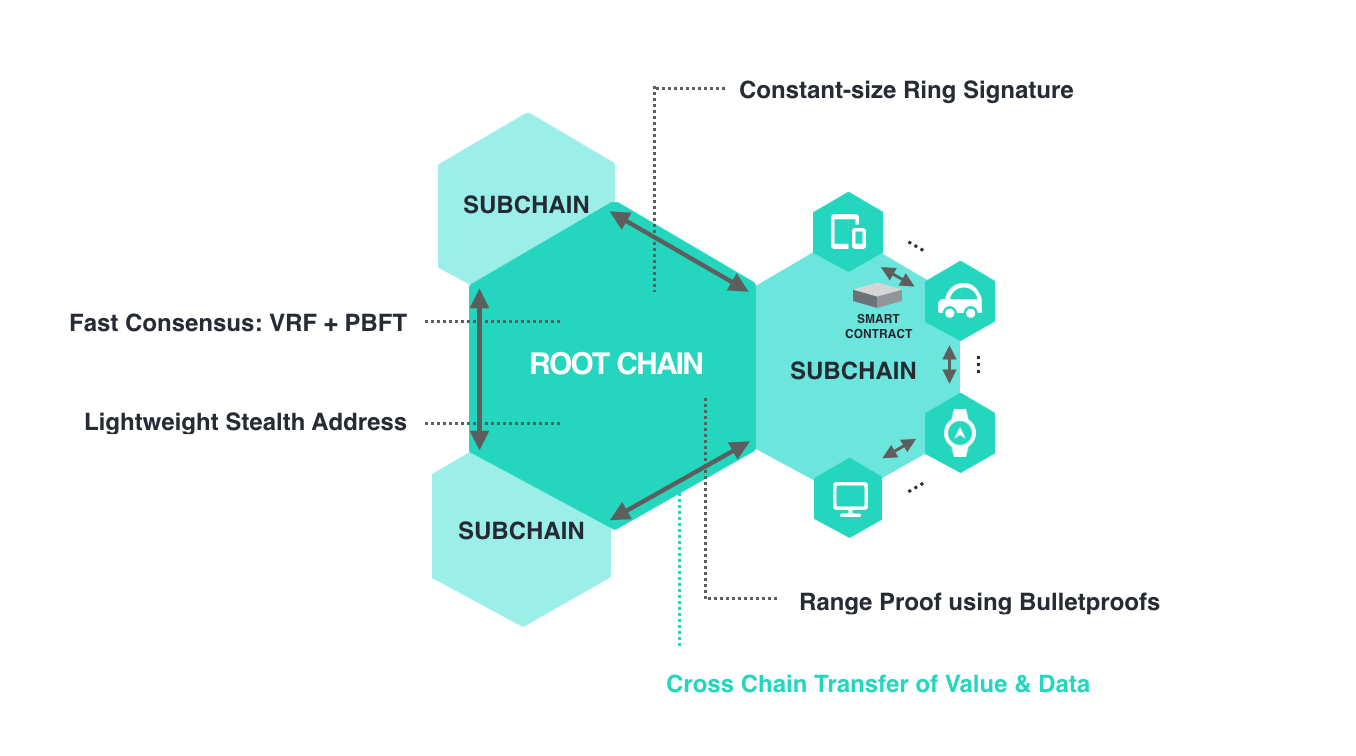
\includegraphics[width=\textwidth]{Figura1.png}
	\label{fig:fig1}
	\caption{IoTeX: Blockchain in blockchain, un'architettura composta da una rootchain con subchain}
\end{figure}

La blockchain radice è una blockchain pubblica accessibile da chiunque, che ha tre obiettivi principali:

\begin{enumerate}
	\item
	      \textbf{Inoltro} di valore e dati tra le subchain, in grado di preservare la privacy, per abilitare l'interoperabilità tra le subchain;
	\item
	      \textbf{Supervisione} delle subchain, ad esempio per penalizzare operatori di subchain confiscandone il deposito;
	\item
	      \textbf{Regolamento e ancoraggio} dei pagamenti e della fiducia per le subchain.
\end{enumerate}
Definiti questi obiettivi, la rootchain si concentra in particolare su scalabilità, robustezza, funzioni di salvaguardia della privacy e capacità di controllare le subchain.
Una subchain, d'altra parte, potrebbe potenzialmente essere una blockchain dotata di privacy e dipendere dalla rootchain per l'interazione con altre subchain. Una subchain richiede flessibilità ed estensibilità per adattarsi ai diversi requisiti delle diverse applicazioni IoT. Una subchain sarà molto probabilmente gestita da operatori il cui ruolo è subordinato a un sufficiente deposito di garanzia, depositato sulla rootchain. Opzionalmente, il sistema consente agli operatori di nominare uno o più operatori terzi che agiscano per suo conto, con o senza vincoli extra. L'operatore agisce come un client leggero nella rootchain, e come un nodo completo nella subchain per confermare nuovi blocchi.
Nel complesso, le proprietà di rootchain e subchain sono riassunte in Tabella \ref{table:rootchainandsubchains}

\begin{table}[tp]%
	\caption{Confronto tra Rootchain e Subchain}
	\label{table:rootchainandsubchains}\centering %
	\begin{tabular}{l|l|l}
		\hline
		\textbf{Proprietà}          & \textbf{Rootchain}   & \textbf{Subchain}  \\
		\hline
		Pubblica vs Privata         & Pubblica             & Pubblica o Privata \\
		Scalabile                   & Necessario           & Varia              \\
		Robusta                     & Fortemente Richiesto & Richiesto          \\
		Incentrata sulla Privacy    & Richiesto            & Varia              \\
		Estendibilità               & Non-Turing completa  & Turing completa    \\
		Finalità Istantanea Blocchi & Richiesta            & Richiesta          \\
		\hline
	\end{tabular}
\end{table}

\subsection{Blockchain Radice}
La blockchain radice utilizza il modello basato su UXTO come Bitcoin \cite{c21} e Monero \cite{c20} per i seguenti motivi:

\begin{itemize}
	\item
	      L'ordinamento delle transazioni diventa banale, non richiede \emph{nonce} o numeri di sequenza, il che pone richieste minime nei metodi di consenso e permette di elaborare le transazioni in parallelo;
	\item
	      Applicando tecniche esistenti di salvaguardia della privacy come la \emph{ring signature} e \texttt{ZKSNARKs}, diventa possibile nascondere il mittente, il destinatario e l'importo della transazione;
\end{itemize}

La blockchain radice è composta da blocchi collegati da hash, e un blocco è costituito da  un'intestazione che lo collega mediante un hash al blocco precedente, oltre che da una lista di transazioni. La rootchain consente principalmente due tipi di transazione: (1) transazioni di base come \texttt{P2PKH, P2SH, Multisig} e così via, e transazioni avanzate che consentono operazioni tra blockchain come \texttt{BondedRegistration, Lock, ReLock, Reorg} ecc.. Le transazioni confermate vengono aggiunte ad un blocco che ha dimensione dinamica, con limite massimo di 8MB. Il nostro sistema di consenso produce un blocco ogni tre secondi come dettagliato nella prossima sezione. La rootchain è progettata per essere non-Turning-Completa, supportata uno script basato su stack e un ricco set di operazioni.

\subsection{Subchain}
IoTeX fornisce un framework per lo sviluppo e la fornitura di una subchain su misura per applicazioni IoT decentralizzate, incapsulando primitive a basso livello come il protocollo gossip ed il meccanismo di consenso. Il modello di autorizzazione, le specifiche, i parametri e i tipi di transazione della subchain possono essere personalizzati per adattarsi alla propria applicazione.
Le subchain IoTeX utilizzano il modello basato su account, che è più vantaggioso per il tracciamento delle transizioni di stato.
Esistono due tipi di account, similmente a Ethereum: account regolari e contratti. Le transazioni valide vengono aggiunte al blocco, che viene generato dallo stesso meccanismo di consenso della blockchain radice al fine di ottenere lo stesso livello di finalità, e rendere la comunicazione cross-chain più efficiente. Le subchain utilizzano o il token della rootchain, IoTeXtoken, oppure definiscono il proprio token. Il token definito dagli sviluppatori per le subchain può essere distribuito mediante vendita pubblica di token oppure scambiati sui siti di cambio pubblici.
Le subchain supportano smart contract, che vengono eseguiti su una macchina virtuale leggera ed efficiente. Attualmente stiamo valutando Web Assembly (WASM) \cite{c36}, uno standard Web emergente per la creazione di applicazioni Web ad alte prestazioni. WASM è veloce ed efficiente, può essere reso deterministico e dotato di sandbox a seguito di piccole modifiche così come tentato dal progetto EOS \cite{c9}, ma vengono esaminate anche altre opzioni. Grazie agli smart contract, i dispositivi IoT collegati alla stessa subchain usano lo stato condiviso in due modi:

\begin{itemize}
	\item Innanzitutto, i dispositivi possono interagire con l'ambiente fisico in base agli stati presenti nella loro subchain, ad es. le lampadine si accendono o spengono autonomamente in base allo stato di un orologio sulla stessa subchain;

	\item D'altra parte, i dispositivi possono cambiare il proprio stato sulla subchain quando l'ambiente fisico cambia, ad esempio, il termostato aggiorna la temperatura tramite uno smart contract in base ai dati provenienti dal suo sensore di temperatura;
\end{itemize}

\subsection{Comunicazione cross-blockchain}
Ci si aspetta che la comunicazione tra blockchain diverse sarà utilizzata di frequente nelle applicazioni IoT. C'è sempre la necessità per un dispositivo IoT in una subchain di coordinarsi con un altro dispositivo in una diversa subchain. Ancora una volta, limitati dalla bassa potenza di calcolo e dal poco spazio di archiviazione dei dispositivi IoT, siamo motivati a progettare un tipo di comunicazione cross-chain che sia veloce ed economica in termini di risorse.

\subsubsection{Pegging e Finalità dei Blocchi}
Il Pegging è un meccanismo per scalare la rete Bitcoin tramite \emph{"sidechain"}, originariamente
proposto in \cite{c1}. Esso si affida fortemente al \emph{Simplified Payment Verifcation} (SPV) \cite{c21}, e consente ai Bitcoin di \"spostarsi\" in modo efficiente dalla blockchain Bitcoin a una sidechain
e viceversa. L'idea alla base è semplice: i token vengono inviati ad un indirizzo speciale al fine di essere bloccati sulla blockchain Bitcoin; una volta confermata questa transazione di \texttt{Lock}, si invia la transazione \texttt{Reorg} alla sidechain, includendo il riferimento alla transazione di \texttt{Lock} ed una prova di inclusione (\emph{"Proof of inclusion"}), sotto forma di ramo Merkle. La sidechain usa il SPV per verificare la transazione di \texttt{Reorg} e, se convalidata, crea una quantità di token equivalente e li invia all'indirizzo desiderato sulla sidechain. Ad oggi, il pegging funge da
primitiva per quasi tutti i protocolli di comunicazione cross-blockchain, ad es. Cosmos, Lisk,
Rootstock. Due flussi separati di pegging possono essere facilmente accoppiati insieme per creare il
cosiddetto Pegging a due vie (2WP) che renalizza il trasferimento di token in entrambi i versi.

La finalità dei blocchi rappresenta la garanzia che ogni nuovo blocco generato sia "finale", e non possa più essere
modificato. La finalità dei blocchi ha un impatto sostanziale sull'attuazione concreta del pegging,
poiché è necessario aspettare fino a che la finalità di un blocco venga raggiunta (almeno con un'alta probabilità) sulla blockchain da cui si invia, prima di richiedere la \texttt{Reorg}. La maggior parte delle blockchain pubbliche come Bitcoin non hanno finalità istantanea. La blockchain ricevente può solo ottenere una sicurezza statistica, poiché man mano che i miners PoW confermano una stessa transazione, aumenta la probabilità che essa sia stata accettata nella blockchain. Utilizzare un consenso con finalità risolve questo problema perché la blockchain ricevente ha la garanzia certa già con la conferma di un solo blocco sulla blockchain inviante. Per le applicazioni IoT, il trasferimento tra le blockchain di valore e dati dovrebbe essere veloce e richiedere poche risorse, e questo impone un meccanismo di consenso con finalità sia sulla rootchain che sulle subchain. Il consenso IoTeX raggiunge la finalità istantanea dei blocchi, come dettagliato nella prossima sezione.

\subsubsection{Protocollo di comunicazione crosschain}
Esaminiamo il protocollo ad alto livello immaginando che un indirizzo di nome \emph{Charlie} sulla
subchain 1 desideri inviare una transazione a un indirizzo di nome \emph{David} sulla subchain 2, e tutte e tre le blockchain usino lo stesso tipo di token, per semplicità senza costi di transazione. Si noti che applicando semplicemente il pegging, saranno necessarie quattro transazioni per effettuare una "remote call" dalla subchain 1 alla subchain 2 attraverso la rootchain, cioè: (1) una transazione di \texttt{Lock} sulla subchain 1; (2) una transazione di \texttt{Reorg} verso la rootchain; (3) un'altra transazione di \texttt{Lock} sulla rootchain; e (4) un'altra transazione di \texttt{Reorg} verso la subchain 2.
Questo processo indica che \emph{David} deve attendere almeno 4 blocchi prima di accettare la "remote call", e i dati che essa trasporta devono essere archiviati su tutte e tre le blockchain, cosa che la rende lenta e costosa. Miriamo a ottimizzare questo processo combinando (2) e (3) in un'unica transazione di \texttt{ReLock}, che non solo accelera l'intero processo ma
evita anche di archiviare i dati nella subchain 1 e nella rootchain. Il nostro protocollo è raffigurato nella Figura \ref{fig:fig2}

\begin{figure}[ht]
	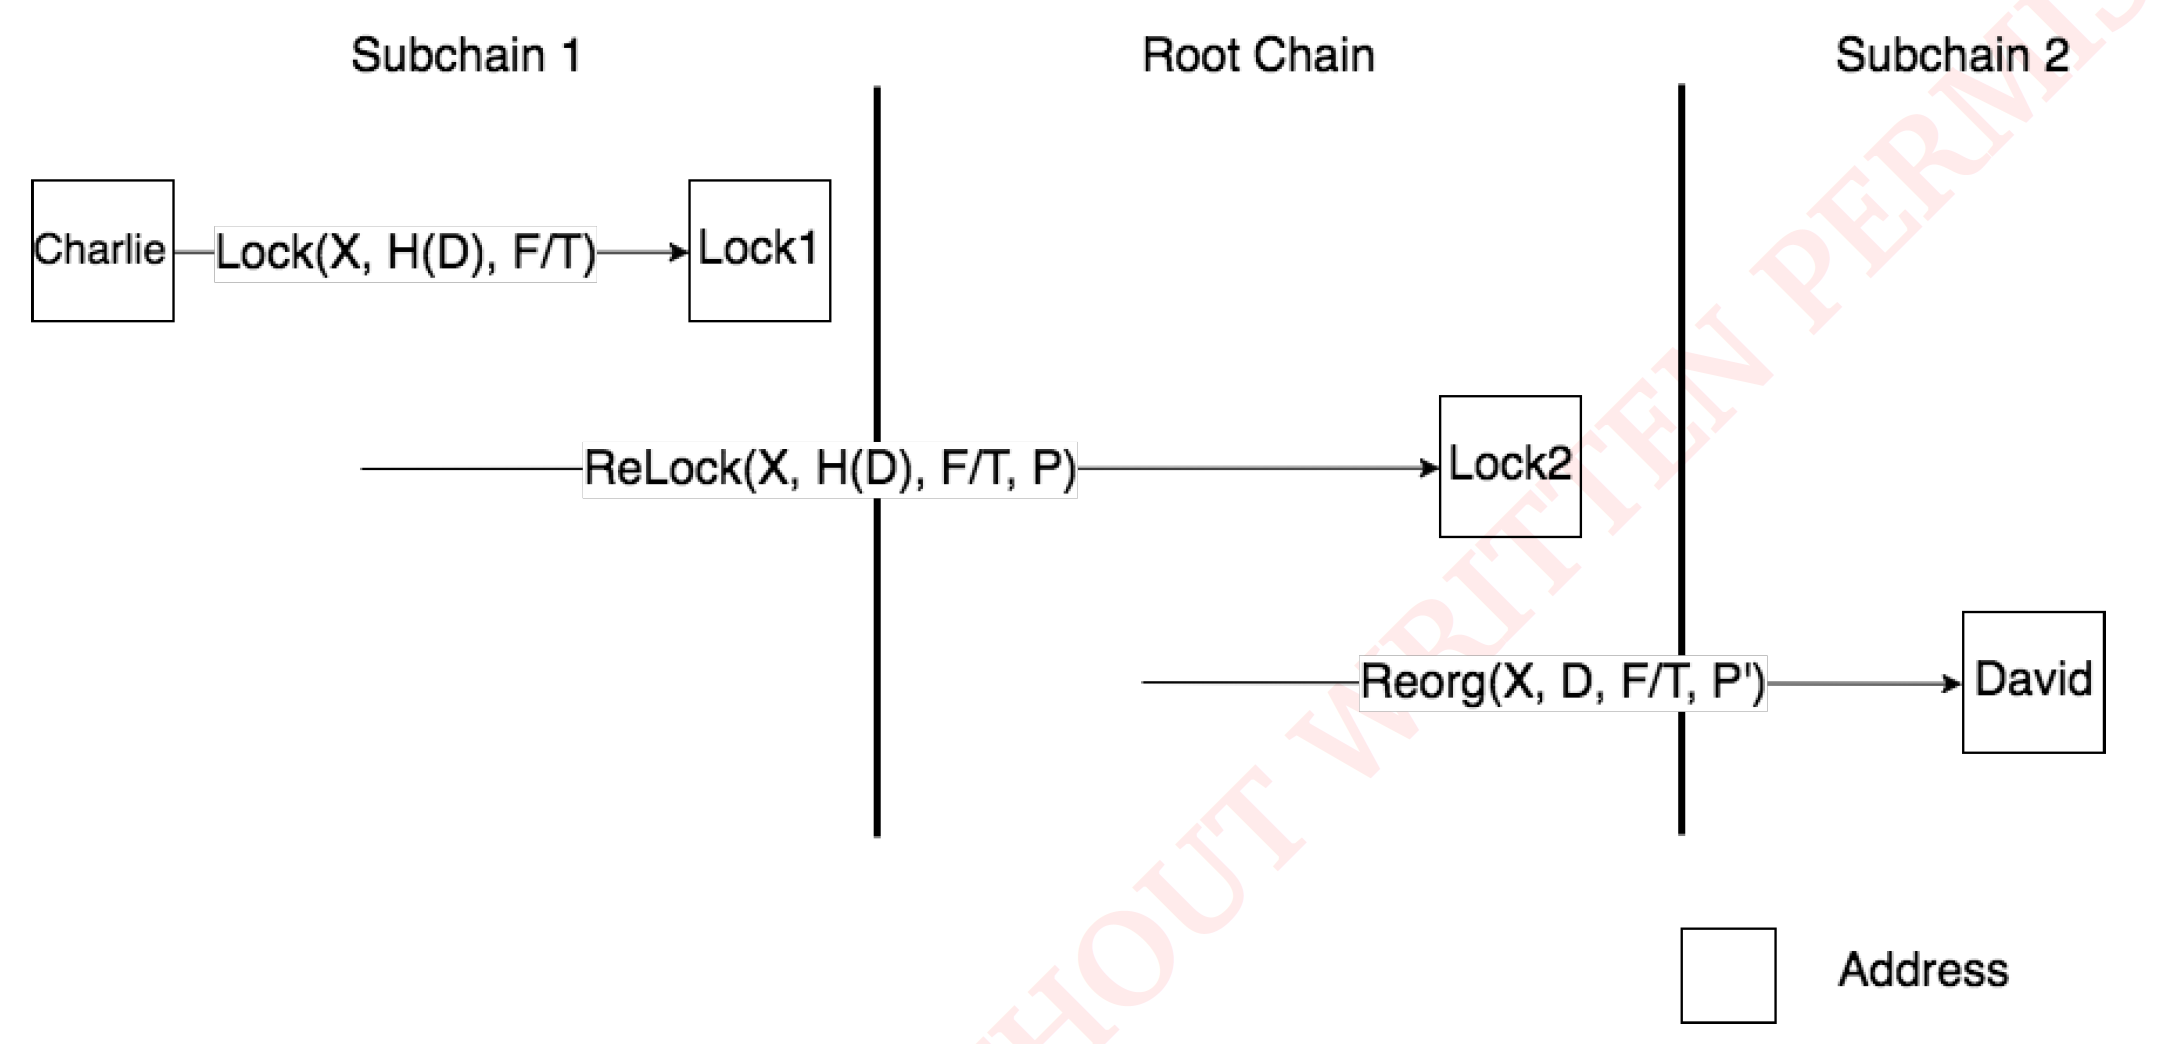
\includegraphics[width=\textwidth]{Figura2.png}
	\label{fig:fig2}
	\caption{Transazioni Cross-Bockchain}
\end{figure}

Il protocollo cross-chain di IoTeX risulta composto dai seguenti passi:

\begin{itemize}
	\item Ogni subchain viene registrate sulla rootchain inviando una transazione chiamata \texttt{BondedRegistration} alla rootchain, che include il nome della subchain, l'ID, la configurazione, il blocco di "genesi", e la nomenclatura degli operatori; questo processo avviene una sola volta;

	\item Quando \emph{Charlie} vuole inviare una transazione a \emph{David}, egli inizia una transazione $\texttt{Lock}(X, H(D), F/T)$ dove $X$ è la quantità di token, $H(D)$ è l'hash dei dati $D$ da allegare, $F/T$ indica gli indirizzi sorgente e destinazione inclusi gli ID per entrambe le subchain;

	\item Una volta che la transazione di \texttt{Lock} è stata inclusa nella blockchain 1, \emph{Charlie} inizia una transazione $\texttt{ReLock(X, H(D), F/T, S, P)}$ con la rootchain includendo $X, H(D), F/T$, alcune statistiche correnti della subchain 1 indicate con $S$ e una "\emph{proof-of-inclusion}" $P$ che comprende i rami Merkle delle intestazioni di blocchi recenti e rami Merkle che provano che la transazione \texttt{Lock} è stata inclusa;

	\item La rootchain valida la transazione \texttt{ReLock}, la accetta includendola nell'ultimo blocco e crea $X$ token bloccandoli in un indirizzo speciale;

	\item Una volta che la transazione \texttt{ReLock} è stata inclusa nella rootchain, \emph{Charlie} invia una transazione $\texttt{Reorg}(X, D, F/T, P')$ sulla rete della rootchain con $X, D, F/T$ ed un'altra \emph{proof-of-inclusion} $P'$ che prova l'inclusione della transazione \texttt{ReLock};

	\item Gli operatori della subchain 2 si accorgono della transazione \texttt{Reorg}, dunque validano e creano la stessa quantità di token sulla subchain 2, inviandoli all'indirizzo di \emph{David} con associati i dati $D$.

\end{itemize}

\subsubsection{Condivisione della larghezza di banda della Blockchain Root}
Una possibile proeccupazione che riguarda la comunicazione crosschain, è che alcune subchain malevoli possano generare \emph{spam} sulla rootchain o su un'altra subchain trasmettendo un'enorme quantità di transazioni crosschain, ed esaurendo così la capacità dell'altra blockchain. Un modo di attenuare il problema è di fare in modo di appaltare ad ogni subchain la propria quota di transazioni, e di limitare la frequenza delle transazioni provenienti da una subchain se la sua quota si esaurisce.

\begin{figure}[ht]
	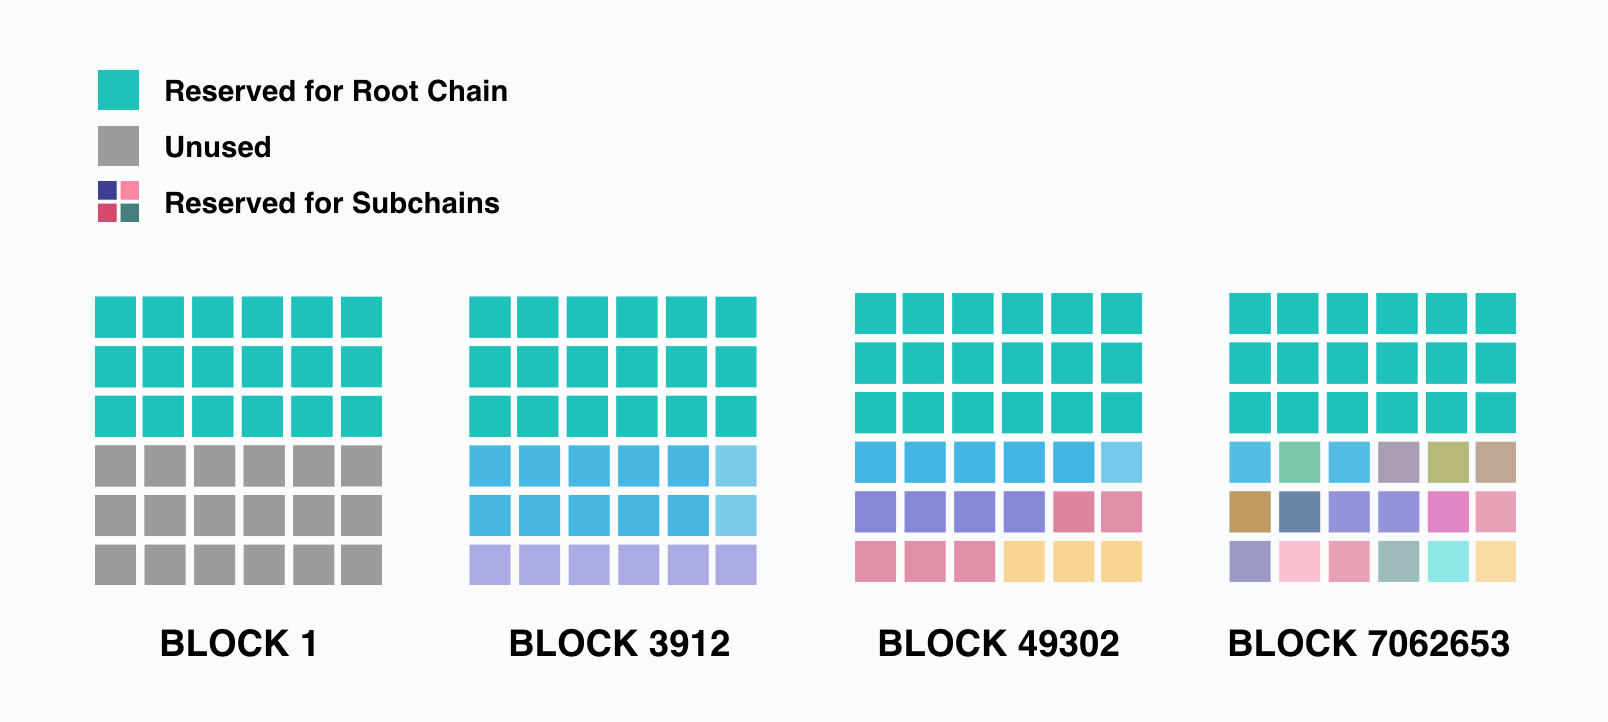
\includegraphics[width=\textwidth]{Figura3.png}
	\label{fig:fig3}
	\caption{Modello della Largezza di Banda per Condividere la Capacità della Rootchain}
\end{figure}

Si potrebbe definire una quota basandosi sullo spazio all'interno di un blocco. Supponiamo che la dimensione massima di un blocco sia di 8MB, e che 4MB siano riservati per le normali transazioni all'interno della rootchain, mentre 4MB siano riservati per tutte le transazioni cross-blockchain, ulteriormente suddivisi in, diciamo 4096 parti di quota, con ogni parte di 1KB. Una subchain richiede l'allocazione $n$ parti di quota (con un limite massimo prefissato) per gli usi desiderati, versando una cauzione proporzionale ad $n$. Ad ogni ciclo, solo $n$KB possono essere occupati all'interno di ciascun blocco per le transazioni provenienti da quella subchain e per ognuna di esse viene scalata una "commissione di banda" dal deposito (per premiare i miner che aiutano ad applicare questa regola); le transazioni rimanenti vengono accodate e, alla fine, scartate quando scadono. L'allocazione delle quote può essere dinamica nel senso che può subire cambiamenti quando la rootchain cresce, come mostrato in Figura \ref{fig:fig3}. Se una subchain inviasse spam alle altre, consumerebbe il proprio deposito molto velocemente ed alla fine perderebbe la propria quota di banda. D'altra parte, se una subchain versasse un grosso deposito esclusivamente al fine di riservare una gran parte di larghezza di banda senza in realtà utilizzarla, la rootchain avrebbe un meccanismo per risarcire parte del deposito secondo il rapporto tra il numero medio di transazioni per blocco e la porzione di banda riservata, il che aiuta a stabilizzare la larghezza di banda riservata ad un valore vicino a quella attualmente utilizzata.